\section{Performance Evaluation}
\label{sec:perf}

In this section, we shall first detail the experimental setting, and we then present the evaluation result and analysis, showing the benefit of \sys{} against state of the art approaches.

\subsection{Experimental Setting}

Experiments were run on a machine with two Intel Xeon E5C2630 2.4GHz CPUs and 64 GB of Memory, running 64 bit Windows 7 professional system.
%
We have employed a real-world dataset Sina Weibo that consists of 24 million microblogs that are associated with 43.5K users.

With respect to the parameters of \sys{}, we use the default values as mentioned in previous sections.
Particularly, for the Feature Extraction module, for practical reasons, we employed a smaller testing dataset to obtain the proper value of $\alpha$ for extracting \textit{Interest Feature};
For the User Cluster module, we studied the clustering solutions with the minimum/maximum number of clusters 2 and 10;
For the Behavior Modeling module, the recent 30 days microblogs of users are used for their short-term interest analysis,
and popular words in the latest 24 hours are returned by Ring as the Hot Event keywords \cite{IEEEexample:ring}.

\subsection{Result and Analysis}
Next, we shall report the performance of system \sys{} over each component.

\stitle{Exp-1: Feature Extraction}
%
Fig.\ \ref{fig:fe} shows the testing results of using various $\alpha$ values.
System \sys{} reaches the optimal results when $\alpha$ is 0.7,
upon which the interest feature extracting is performed for the overall dataset with 43.5K users and 24 million microblogs.
In general, it performs well when $\alpha$ falls into $[0, 0.8]$.




\stitle{Exp-2: User Clustering}
%
Fig.\ \ref{fig:uc} depicts the Silhouette Coefficient Values of multiple clustering solutions, with the cluster number varied from 2 to 10.
Specially, we used different testing datasets, with \textit{Data} containing the overall 43.5K users, and each of \textit{\{Data1,\ldots, Data5\}} contains 10K randomly selected users.
Except for \textit{Data1}, solutions for \textit{\{Data2,\ldots, Data5\}} are the best for 4 clusters.


\begin{figure}[tb!]
\centering
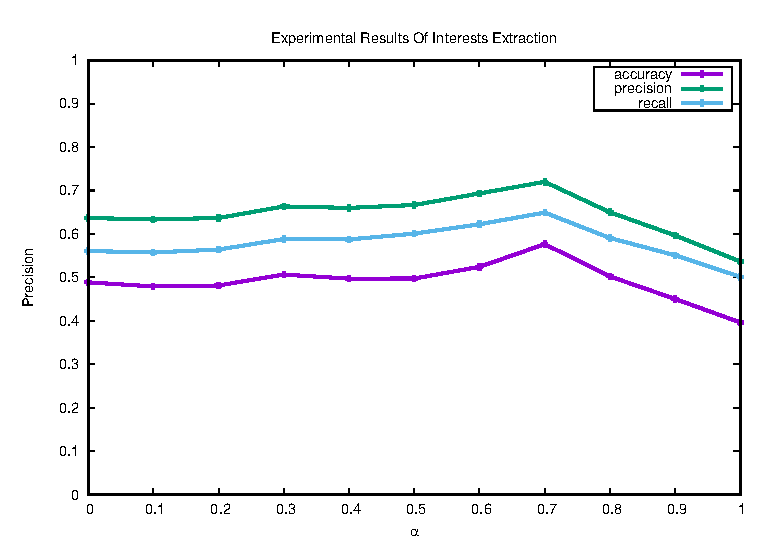
\includegraphics[width=.7\linewidth]{figures/Interests}
\caption{Testing Results with Various $\alpha$.}
\label{fig:fe}
\vspace{-1ex}
\end{figure}

\begin{figure}[tb!]
\centering
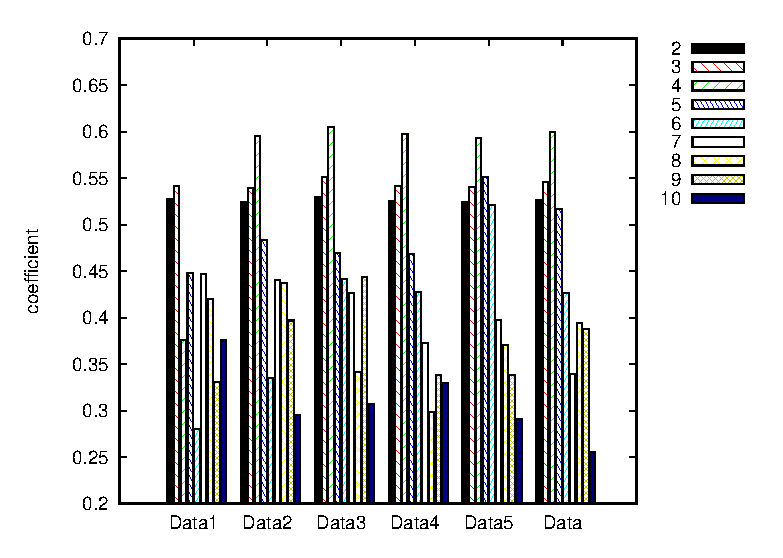
\includegraphics[width=.85\linewidth]{figures/clustering}
\caption{Silhouette Coefficient Values for Various Cluster Numbers over Different Testing Datasets.}
\label{fig:uc}
\vspace{-2ex}
\end{figure}


\begin{figure*}[tb!]
  \centering
  \subfigure[Precision]{
    \label{fig:10-a}
    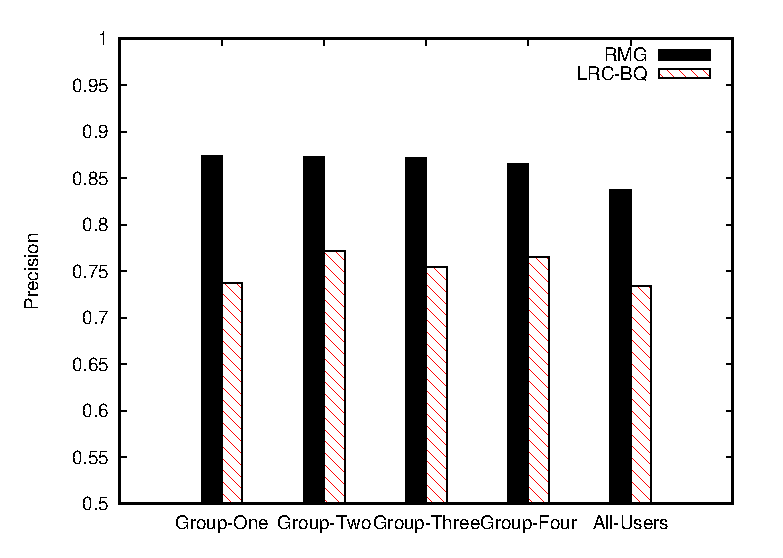
\includegraphics[width=0.32\textwidth]{figures/precision.eps}}
  %\hspace{1in}
  \subfigure[Recall]{
    \label{fig:10-b}
    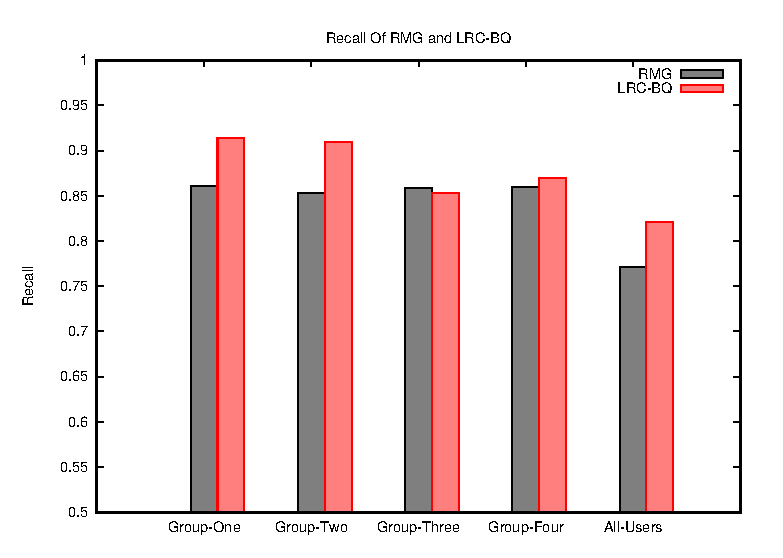
\includegraphics[width=0.32\textwidth]{figures/recall.eps}}
  %\hspace{1in}
  \subfigure[$F_1$ Score]{
    \label{fig:10-c}
    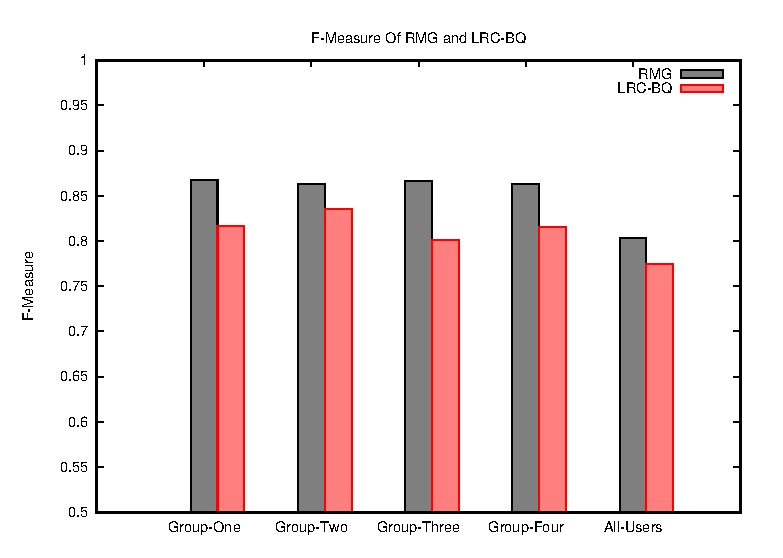
\includegraphics[width=0.32\textwidth]{figures/F-Measure.eps}}
  \caption{Performance of \sys{} Versus LRC-BQ.}
  \label{fig:10}
\end{figure*}


\stitle{Exp-3: Behavior Modeling}
%
Fig.\ \ref{fig:10} shows the performance of \sys{} against the state of the art approach LRC-BQ \cite{IEEEexample:conf/ijcai/ZhangLTCL13}.
We evaluate the performance using the metrics of precision, recall, and $F_1$ score.
LRC-BQ does not deal with user grouping.
Hence, we not only study the modeling effect per group (i.e., ``Group-One/Two/Three/Four'' with user clustering),
but also examine \sys{} versus LRC-BQ in the case that all users are in a single group (i.e., ``All-Users'').
The results show that:
%\begin{itemize}

	\stab(1) With user clustering, \sys{} performs better than LRC-BQ in most cases.
	
	\stab(2) For \sys{}, having user clustering is better than the alternative mono group. Ditto for LRC-BQ.
%\end{itemize}





Fig.\ \ref{fig:11} explores the performance of \sys{} when using alternative data items for modeling.
By default, \sys{} uses ``UI+II+MI'', i.e., items of users (UI), microblogs (MI) and interactions (II).
How about using other combinations of the above item(s)?
As shown in Fig.\ \ref{fig:11}, the default setting wins in most cases.

\begin{figure*}
  \centering
  \subfigure[Precision]{
    \label{fig:11-a}
    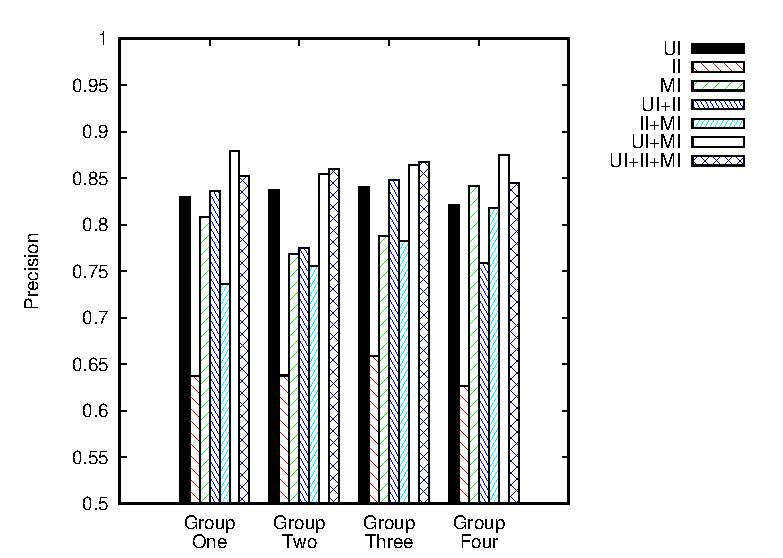
\includegraphics[width=0.32\textwidth]{figures/precisionofdifferentfeatures.eps}}
  %\hspace{1in}
  \subfigure[Recall]{
    \label{fig:11-b}
    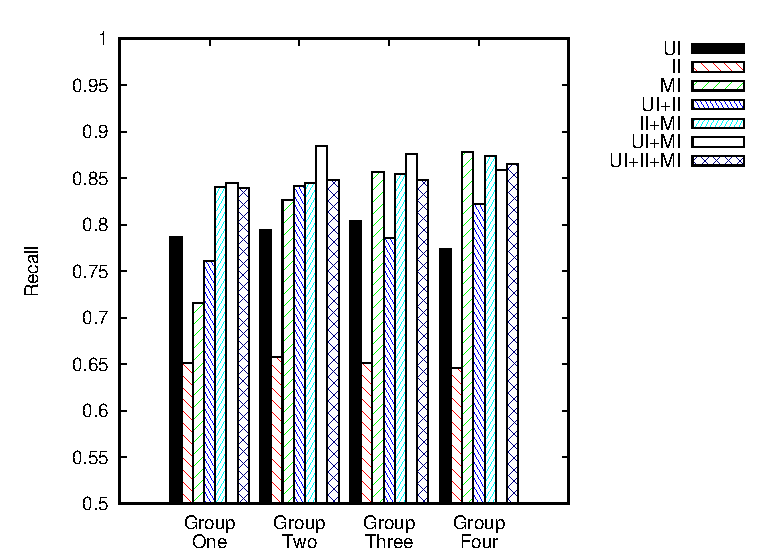
\includegraphics[width=0.32\textwidth]{figures/recallofdifferentfeatures.eps}}
  %\hspace{1in}
  \subfigure[$F_1$ Score]{
    \label{fig:11-c}
    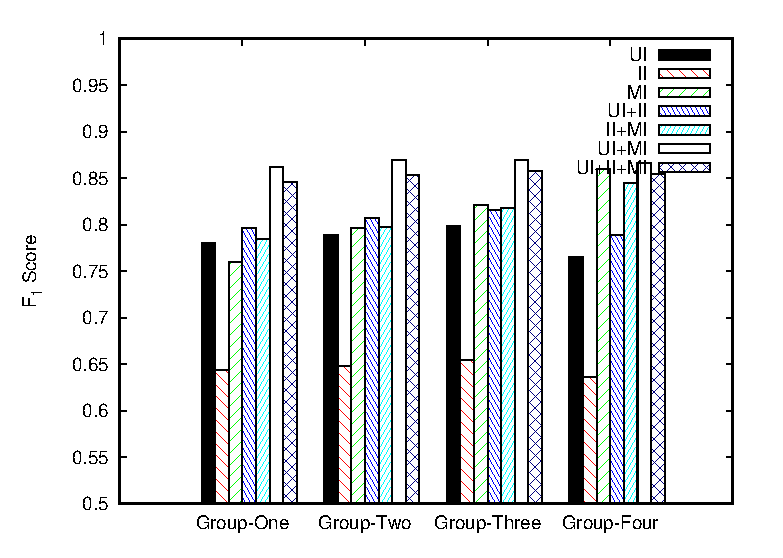
\includegraphics[width=0.32\textwidth]{figures/fmeasureofdifferentfeatures.eps}}
  \caption{\sys{} Performance of Using Various Data Items for Modeling.}
  \label{fig:11}
  \vspace{-1ex}
\end{figure*}

\stitle{Exp-4: Case Study for Feature Extraction}
In this test, we show the results of our demo system for user features extraction.
%
Considering the huge amount of users, we carefully selected one typical user for analysis.
Here we chose Mary (a famous drama and movie actress in China) as an example.

The feature extraction result for Mary is depicted in Fig.\ \ref{fig:userFeatures}.
Then we can see the basic information of Mary in Fig.\ \ref{fig:userFeatures:uf-1}: her nickname is Actress Mary (��Ա����) and she is from Beijing (����).
Mary has more followers than followees.
The Sina Microblog tag she made for herself is ``actress'' (��Ա).
As to the long-term interest, she is interested with stage performance (��̨����), drama (�������),film (��Ӱ��Ӱ) and so on as shown in Fig.\ \ref{fig:userFeatures:uf-2}, which is consistent with her tag.
The probability distribution of tweeting and retweeting indicates that she is more active at night than daytime as shown in Fig.\ \ref{fig:userFeatures:uf-3} and \ref{fig:userFeatures:uf-4}.
According to Fig.\ \ref{fig:userFeatures:uf-5} and \ref{fig:userFeatures:uf-6}, the interval between her two tweeted/retweeted microblogs is mostly within 48 hours, showing she is an active user.
Mary's short-term interest, e.g. from 09/01/2016 to 09/30/2016, is shown in Fig.\ \ref{fig:userFeatures:uf-7}, which indicates she had been busy with promoting the drama ``Earl of Oolong Mountain'' (����ɽ����). So the results are in line with expectations, as drama (����) and stage (��̨) in Fig.\ \ref{fig:userFeatures:uf-7}.

\begin{figure*}
  \centering
  \subfigure[]{
      \label{fig:userFeatures:uf-1}
      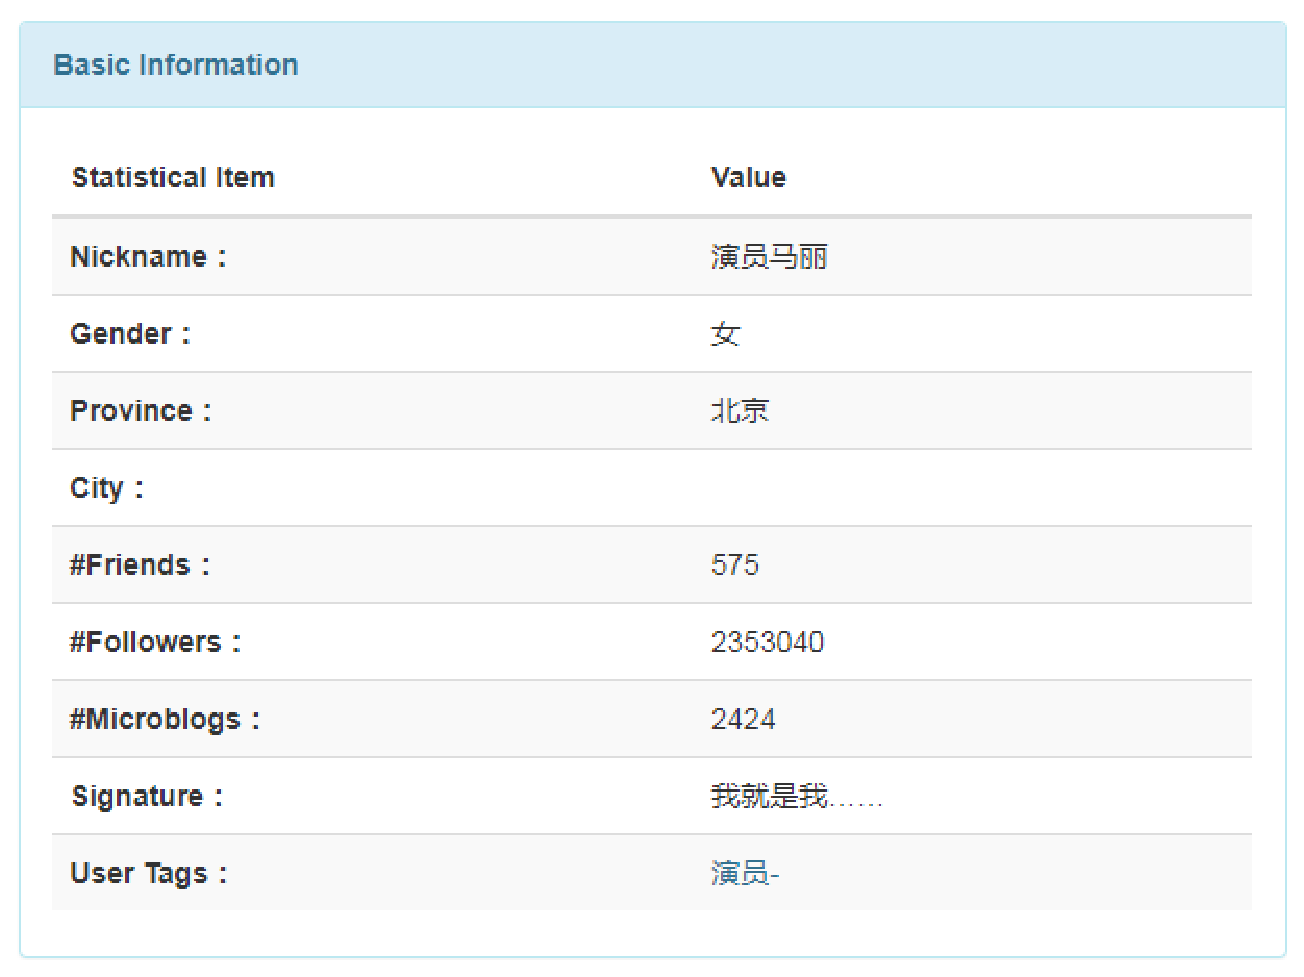
\includegraphics[width=0.23\textwidth]{IMAGE/features/userFeatures/1.eps}}
  \subfigure[]{
      \label{fig:userFeatures:uf-2}
      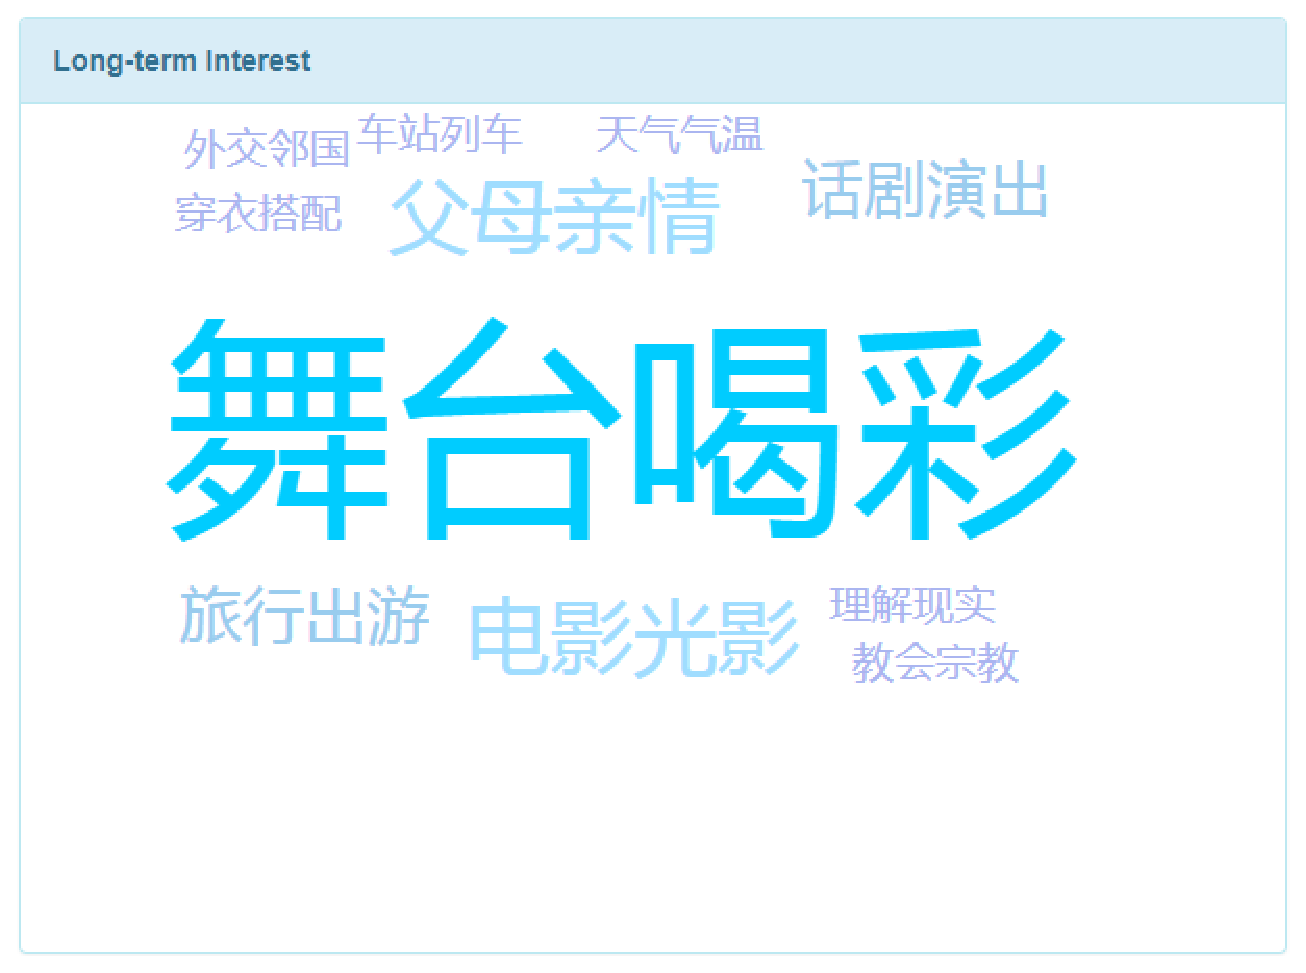
\includegraphics[width=0.23\textwidth]{IMAGE/features/userFeatures/2.eps}}
  \subfigure[]{
      \label{fig:userFeatures:uf-3}
      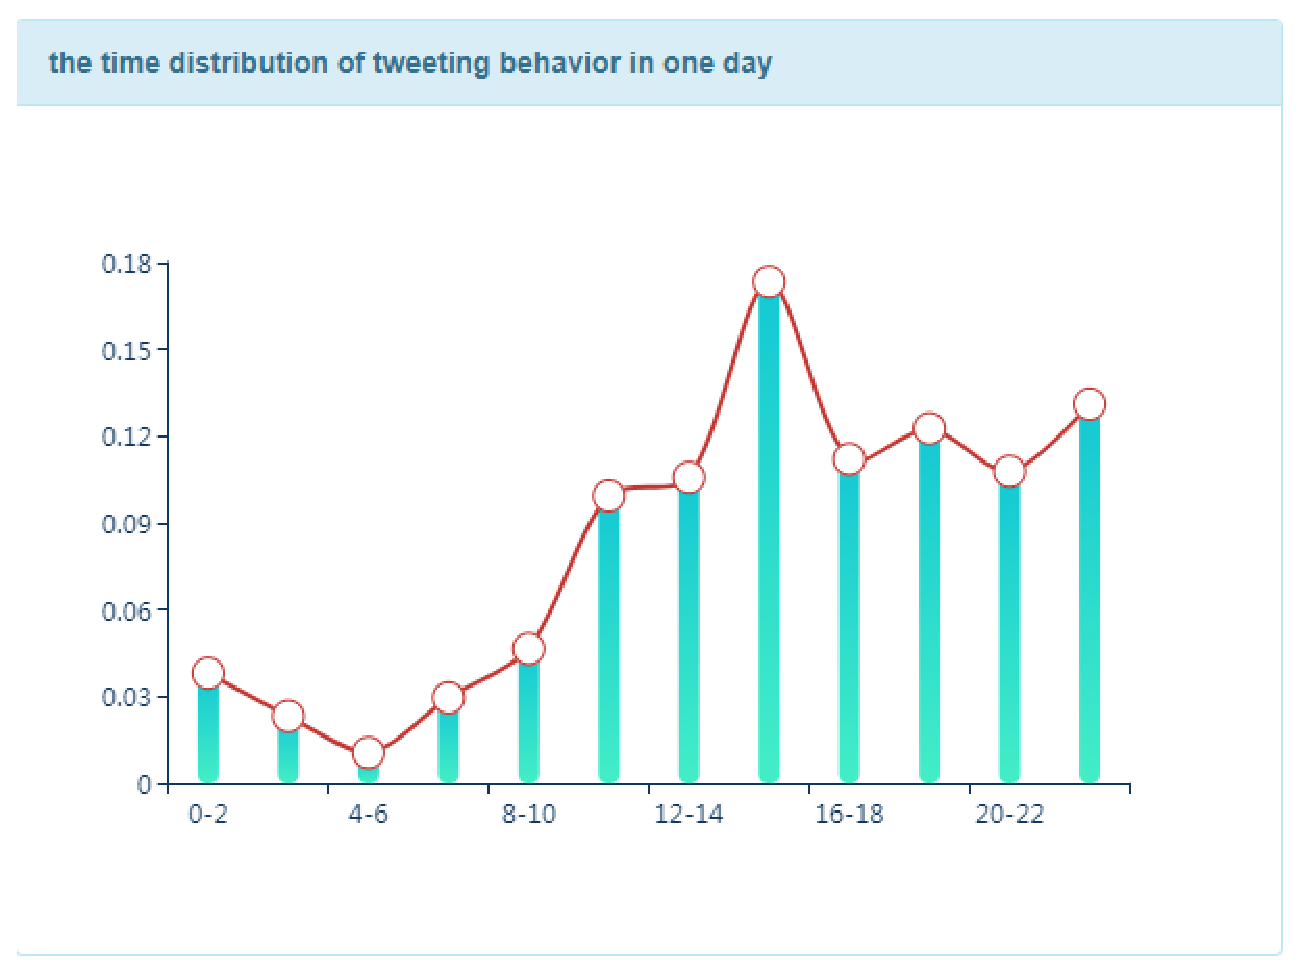
\includegraphics[width=0.23\textwidth]{IMAGE/features/userFeatures/3.eps}}
  \subfigure[]{
      \label{fig:userFeatures:uf-4}
      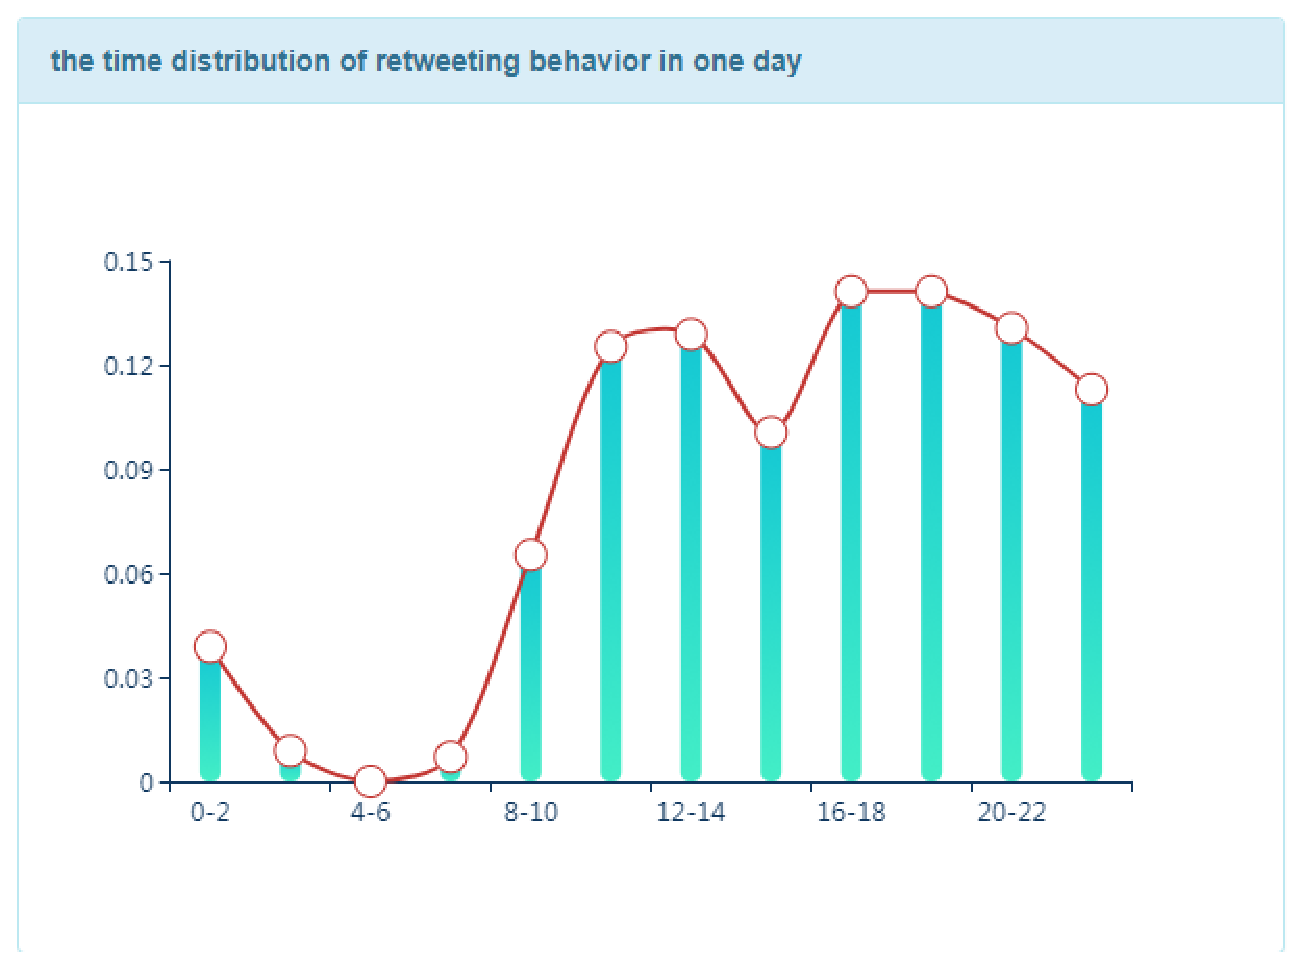
\includegraphics[width=0.23\textwidth]{IMAGE/features/userFeatures/4.eps}}
  \subfigure[]{
      \label{fig:userFeatures:uf-5}
      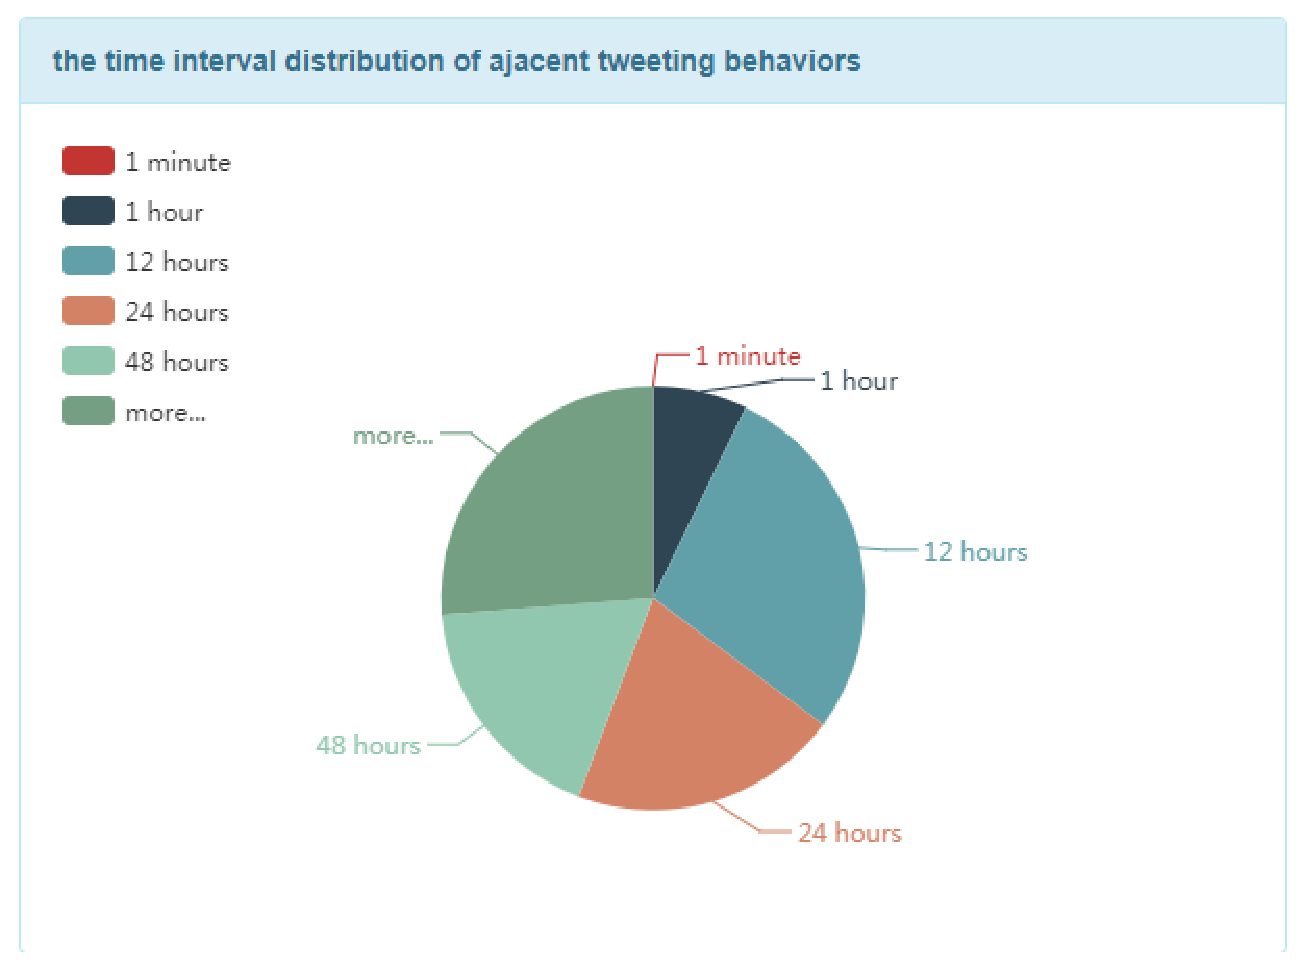
\includegraphics[width=0.23\textwidth]{IMAGE/features/userFeatures/5.eps}}
  \subfigure[]{
      \label{fig:userFeatures:uf-6}
      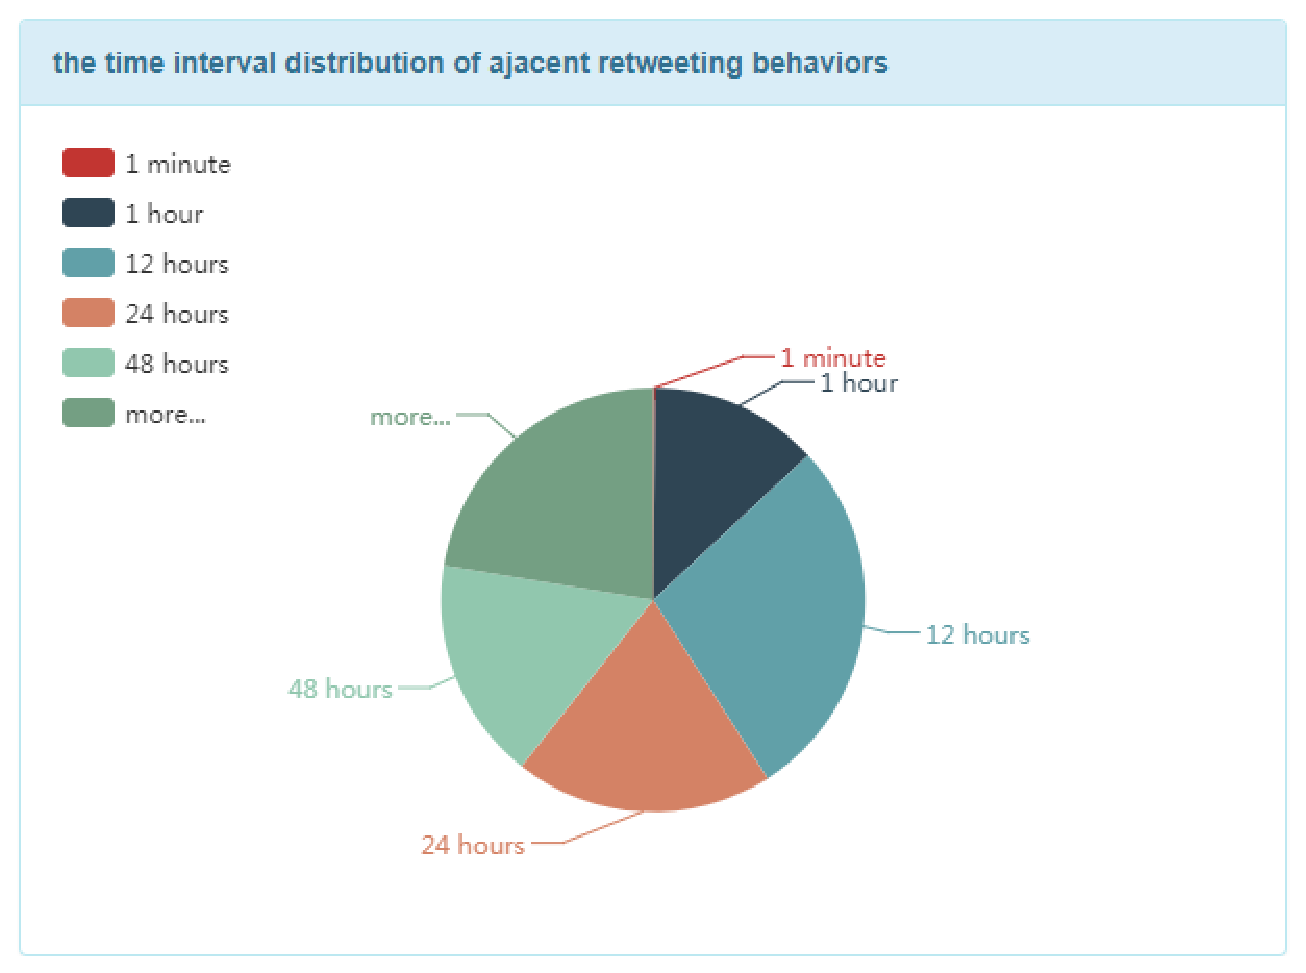
\includegraphics[width=0.23\textwidth]{IMAGE/features/userFeatures/6.eps}}
  \subfigure[]{
      \label{fig:userFeatures:uf-7}
      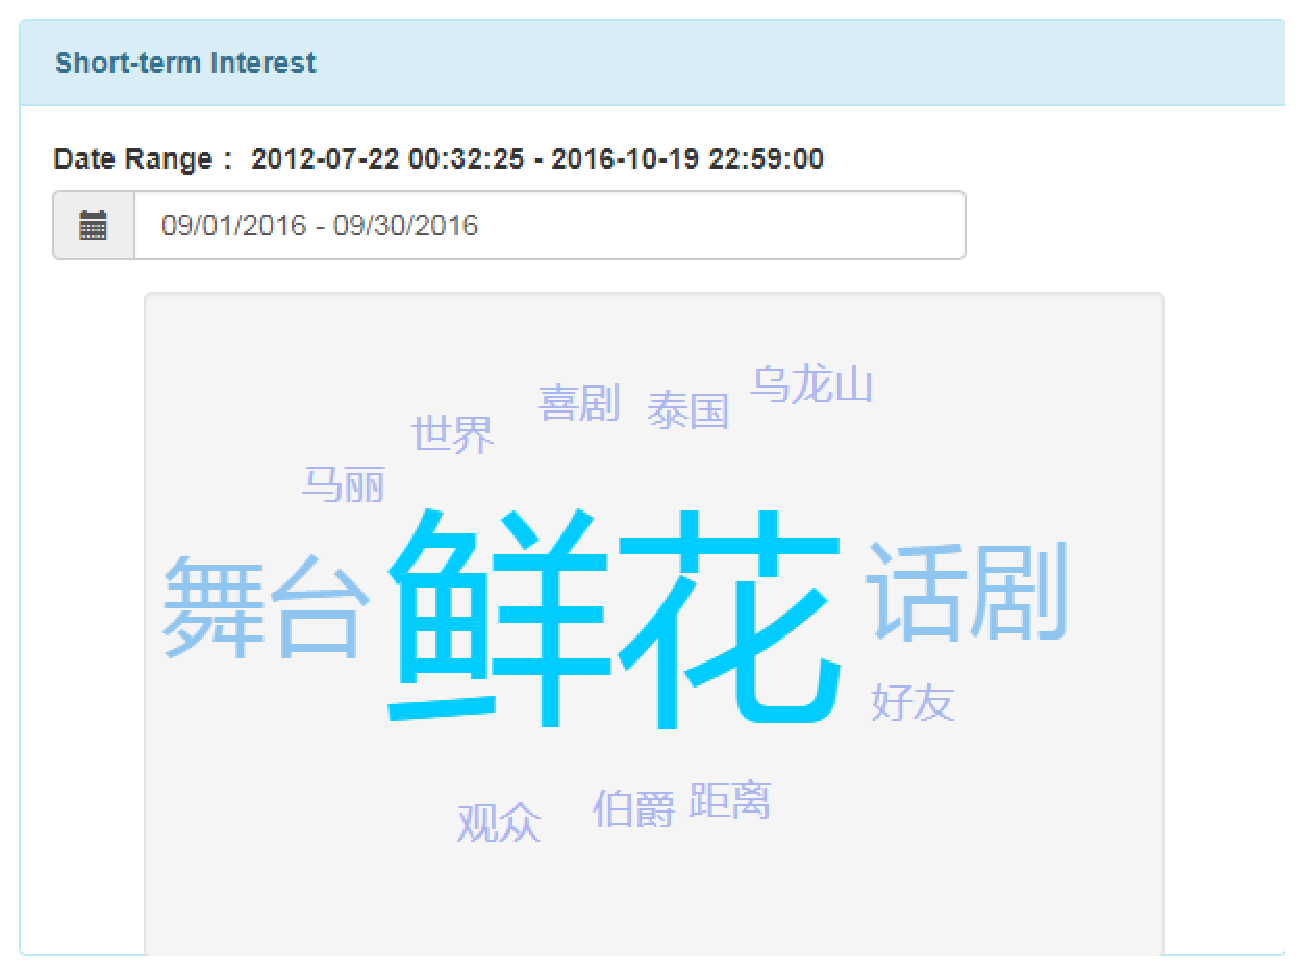
\includegraphics[width=0.23\textwidth]{IMAGE/features/userFeatures/7.eps}}
  \subfigure[]{
      \label{fig:userFeatures:uf-8}
      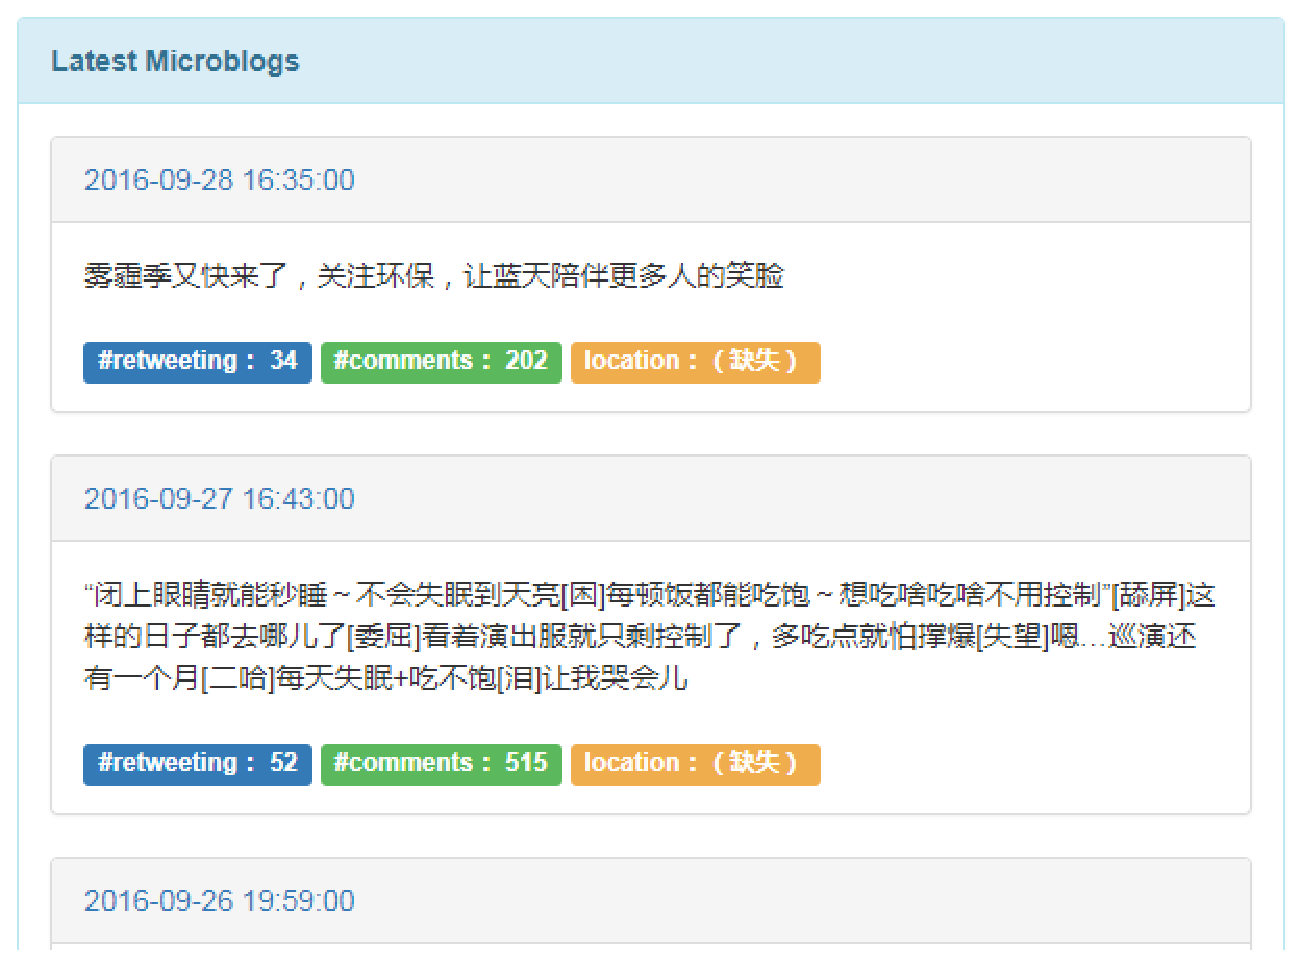
\includegraphics[width=0.24\textwidth]{IMAGE/features/userFeatures/8.eps}}
  \caption{Visualization for User Features.}
  \label{fig:userFeatures} %% label for entire figure
\end{figure*}
